\section{Schémas Numériques}
On a le modèle suivant (``KPP avec mémoire"): 
\begin{equation} \left\{
                \begin{array}{ll}
                   \dt\mu = K\Delta\mu + C(\mu + \rho) -\mu\rho\\
                 \dt\rho=  F_0 \mu \\
                  \dt C = -b\rho C
                \end{array}
              \right.
\end{equation}
\subsection{Pour l'équation différentielle ordinaire}
Sans dépendance spatiale:
\begin{equation} \left\{
                \begin{array}{ll}
                   \dt\mu = C(\mu + \rho) -\mu\rho\\
                 \dt\rho=  F_0 \mu \\
                  \dt C = -b\rho C
                \end{array}
              \right.
\end{equation} 
\subsubsection{Schéma semi-implicite I pour l'EDO}
Soit le schéma semi-implicite I pour l'EDO:
\begin{equation} \boxed{\left\{
                \begin{array}{ll}
                   \mu^{n+1} = \mu^{n}+  \Dt( C^{n}(\mu^{n+1} + \rho^{n+1}) -\mu^{n+1}\rho^{n})\\
                \rho^{n+1}=  \rho^{n}+ \Dt (F_0 \mu^{n+1}) \\
                 C^{n+1} =C^{n}- \Dt(b\rho^{n+1}C^{n+1})
                \end{array}
              \right.}
\end{equation}
Ce schéma donne:
\begin{equation*} \left\{
                \begin{array}{ll}
                   \mu^{n+1}(1-\Dt(C^{n}(1+\Dt F_0)) + \rho^{n}) = \mu^{n}+  \Dt C^{n}\rho^{n} \\
                \rho^{n+1}=  \rho^{n}+ \Dt (F_0 \mu^{n+1}) \\
                 C^{n+1} =C^{n}\frac{1}{1+ \Dt b\rho^{n+1}}
                \end{array}
              \right.
\end{equation*}
\paragraph{Positivité}
Pour conserver la positivité il suffit que le terme $(1-\Dt(C^{n}(1+\Dt F_0)) + \rho^{n}) $ reste positif:\\
Par exemple: 
\begin{equation}
	\boxed{C^0< \frac{1}{\Dt(1+F_0\Dt)}}
\end{equation}

\subsubsection{Schéma semi-implicite II pour l'EDO}
Soit le schéma semi-implicite II pour l'EDO:
\begin{equation} \boxed{\left\{
                \begin{array}{ll}
                   \mu^{n+1} = \mu^{n}+  \Dt( C^{n}(\mu^{n+1} + \rho^{n+1}) -\mu^{n}\rho^{n})\\
                \rho^{n+1}=  \rho^{n}+ \Dt (F_0 \mu^{n+1}) \\
                 C^{n+1} =C^{n}- \Dt(b\rho^{n+1}C^{n+1})
                \end{array}
              \right.}
\end{equation}
Ce schéma donne:
\begin{equation*} \left\{
                \begin{array}{ll}
                   \mu^{n+1}(1-\Dt(C^{n}(1+\Dt F_0))) = \mu^{n}+  \Dt \rho^{n}(C^{n}-\mu^{n}) \\
                \rho^{n+1}=  \rho^{n}+ \Dt (F_0 \mu^{n+1}) \\
                 C^{n+1} =C^{n}\frac{1}{1+ \Dt b\rho^{n+1}}
                \end{array}
              \right.
\end{equation*}
\paragraph{Positivité}
Pour conserver la positivité il suffit que les terme $(1-\Dt(C^{n}(1+\Dt F_0)))$ et $\mu^{n}+  \Dt \rho^{n}(C^{n}-\mu^{n})$ restent positif:\\
Par exemple: 
\begin{equation}
	\boxed{C^0< \frac{1}{\Dt(1+F_0\Dt)}}
\end{equation}
et 
\begin{equation}
	\boxed{\rho^n< \frac{1}{\Dt}}
\end{equation}
On obtient une condition de plus que le schéma semi-implicite I.
\subsection{Pour l'équation aux dérivées partielles}
\subsubsection{Schéma semi-implicite I pour l'EDP}
Soit le schéma semi-implicite I pour l'EDP:
\begin{equation} \boxed{\left\{
                \begin{array}{ll}
                   \mu^{n+1}_i = \mu^{n}_i+ K\Dt \frac{\mu^{n+1}_{i+1}-2\mu^{n+1}_i+\mu^{n+1}_{i-1}}{\Dx ^2} + \Dt( C^{n}_i(\mu^{n+1}_i + \rho^{n+1}_i) -\mu^{n+1}_i\rho^{n}_i)\\
                \rho^{n+1}_i=  \rho^{n}_i+ \Dt (F_0 \mu^{n+1}_i) \\
                 C^{n+1}_i =C^{n}_i- \Dt(b\rho^{n+1}_iC^{n+1}_i)
                \end{array}
              \right.}
\end{equation}
Ce schéma donne:
\begin{equation*} \left\{
                \begin{array}{ll}
                   (1+\frac{K\Dt}{\Dx^2}A-\Dt(C^{n}(1+\Dt F_0)) + \rho^{n})\mu^{n+1} = \mu^{n}+  \Dt C^{n}\rho^{n} \\
                \rho^{n+1}=  \rho^{n}+ \Dt (F_0 \mu^{n+1}) \\
                 C^{n+1} = C^{n}\frac{1}{1+ \Dt b\rho^{n+1}}
                \end{array}
              \right.
\end{equation*}
où $A$ est la matrice de $-\Delta$
:\begin{equation}  \label{myeq}A= \left[ \begin{matrix}2 & -1 & & 0\\-1 & \ddots & \ddots &  \\& \ddots & \ddots &  -1 \\0 &  & -1 & 2  \end{matrix}  \right]\end{equation}
\paragraph{Positivité}
Afin de préserver la positivité, on obtient la même condition (suffisante) que pour l'EDO:
\begin{equation}
	\boxed{C^0< \frac{1}{\Dt(1+F_0\Dt)}}
\end{equation}
\begin{proof} Supposons $\mu^0 >0$.\\ Raisonnons par l'absurde et supposons que $n=\min{n \mid \exists j \mid \mu^{n+1}_j < 0}$ existe. Soit $j = \argmin{\mu^{n+1}_i}$.\\
On a $(1-\Dt(C^{n}_j(1+\Dt F_0)) + \rho^{n}_j)\mu^{n+1}_j = \mu^{n}+  \Dt C^{n} +\frac{K\Dt}{\Dx^2}(\mu^{n+1}_{j+1} - 2\mu^{n+1}_j + \mu^{n+1}_{j-1}) $. \\
Or par définition de $n$ et comme $C^0< \frac{1}{\Dt(1+F_0\Dt)}$ et $C^n < C^0$:\\
 $ \mu^{n}+  \Dt C^{n} > 0$ \\
 $ 1-\Dt(C^{n}_j(1+\Dt F_0)) + \rho^{n}_j > 0$ \\
Et par définition de $j$: \\
$\mu^{n+1}_{j+1} - 2\mu^{n+1}_j + \mu^{n+1}_{j-1} \geq 0$\\
On a donc $\mu^{n+1}_j > 0$ mais   $\mu^{n+1}_j = \min(\mu^{n+1}_i) < 0$ par définition de $j$ et $n$ : C'est absurde.
\end{proof}

\newpage
\section{Résolution numérique}
\subsection{Résolution de l'EDO}
\subsubsection{Résultat de la simulation de l'EDO}
\begin{figure}[hbt!]
\centering
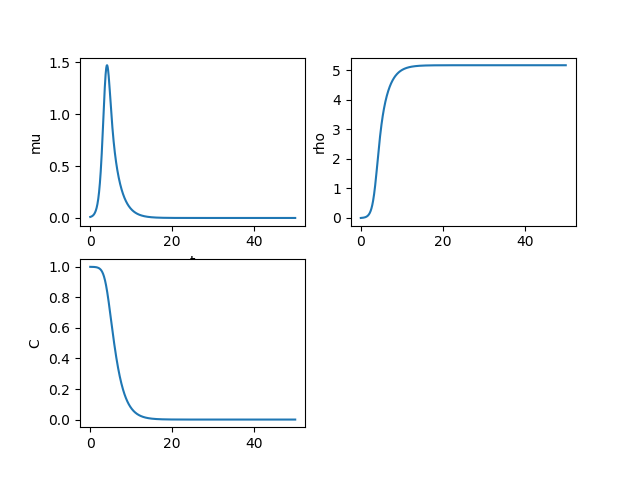
\includegraphics[width=.7\textwidth]{Images/edo_euler_implicite.png}
\caption{Résolution du schéma implicite pour l'EDO}
\end{figure}

\subsubsection{Observations de la simulation de l'EDO}
 On observe les phénomènes attendus sur l'EDO:\\
 -i) $\mu$ est bornée et tend vers 0.\\
 -ii) $\rho$ est croissante et bornée.\\
 -iii) $C$ décroît vers 0.\\
 -iv) Les solutions ont un comportement exponentiel autour des états stationnaires et ce comportement est bien prédit par la linéarisation de l'EDO autour de ces états:

\begin{SCfigure}[][h!]
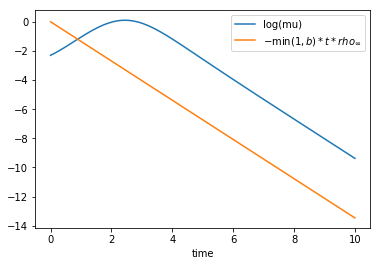
\includegraphics[width=0.4\textwidth]{Images/linearisation.png}
\caption{Comportement de $\log(\mu)$, en particulier autour de $(\mu,\rho,C) =  (0,\rho_\infty,0)$. $\log(\mu)$ est bien linéaire autour des états stationnaires et sa pente (le facteur dans l'exponentielle) correspond exactement à $-\min(1,b)\rho_\infty$ ce qui est un résultat obtenu dans la partie Linéarisation } 
\end{SCfigure} 


\newpage
\subsection{Résolution de l'EDP en 1D}
\subsubsection{Résultat de la simulation de l'EDP en 1D}
\begin{figure}[hbt!]
\centering
\begin{subfigure}[b]{0.45\textwidth}
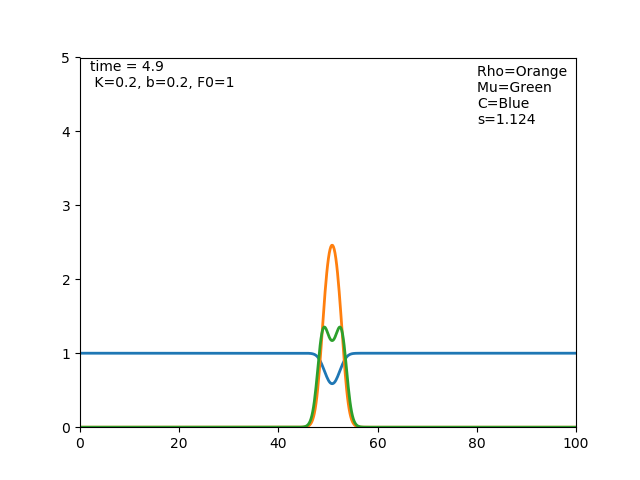
\includegraphics[width=\textwidth]{Images/edp_1d_0.png}
\end{subfigure}
\begin{subfigure}[b]{0.45\textwidth}
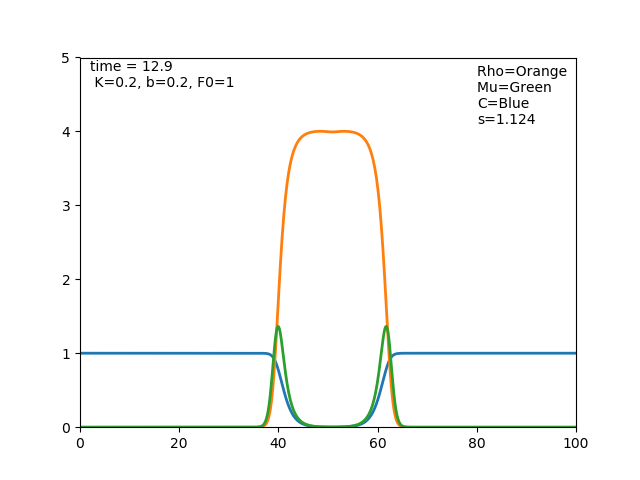
\includegraphics[width=\textwidth]{Images/edp_1d_1.png}
\end{subfigure}
\begin{subfigure}[b]{0.45\textwidth}
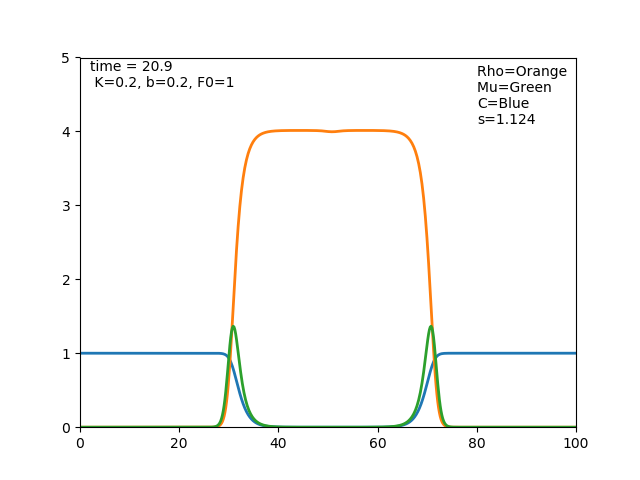
\includegraphics[width=\textwidth]{Images/edp_1d_2.png}
\end{subfigure}
\begin{subfigure}[b]{0.45\textwidth}
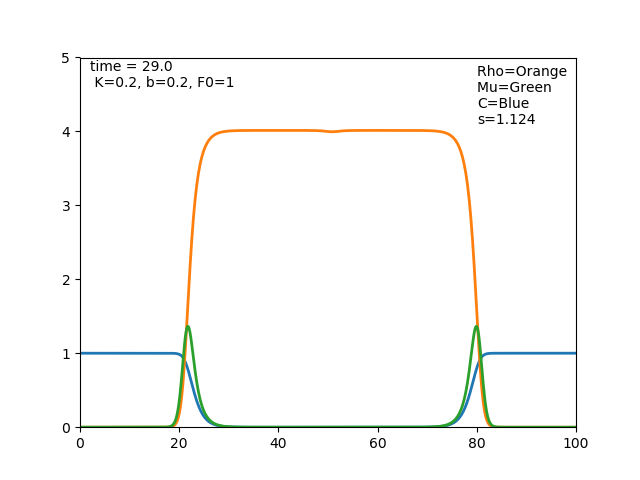
\includegraphics[width=\textwidth]{Images/edp_1d_3.png}
\end{subfigure}
\caption{Résolution du schéma semi implicite I pour l'EDP en 1D} 
\end{figure}
On voit sur les simulations que la solution tend vers une solution de type onde plane stationnaire. Il est possible de calculer cette vitesse et de la comparer avec la vitesse théorique minimale obtenue dans la partie 3: 

\newpage
 
\begin{figure}[hbt!]
\centering
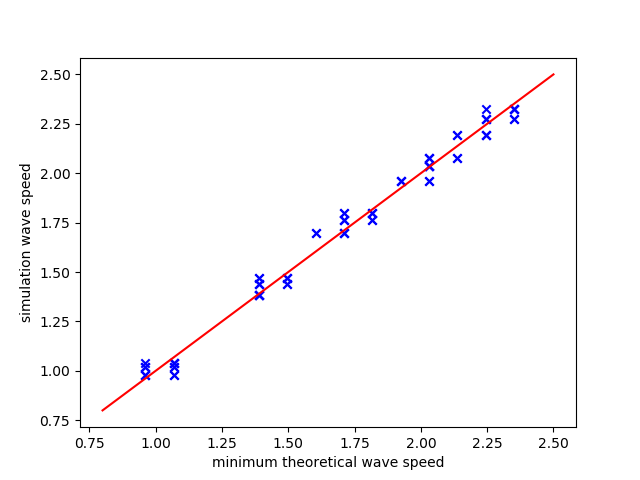
\includegraphics[width=.7\textwidth]{Images/stheoriquevssimulations.png}
\caption{Vitesse du front observée numériquement en fonction de la vitesse minimale théorique}
\end{figure}
Soit \begin{equation*}
s^*_{theorique} =K\frac{f_0(18F_0+4)+\sqrt{f_0(f_0(18F_0+4)^2+108(f_0+4F_0)F_0^2)}}{2(f_0+4F_0)}\end{equation*} la vitesse minimale théorique obtenue dans la partie 3.\\
Ce graphe représente par les points bleus la vitesse du front observée numériquement pour différentes simulations en fonction de la vitesse minimale théorique associée à cette simulation. La droite rouge est la droite $s_{simu} = s^*_{theorique}$.\\
On remarque que la vitesse du front observée numériquement est très proche de la vitesse minimale théorique: ce phénomène est similaire à celui de l'équation de Fisher-KPP: pour une donnée initiale à support compact, \textbf{le front se propage asymptotiquement à la vitesse minimale de l'équation d'onde associée à l'EDP}.